\begin{figure}[h!]
	\centering
	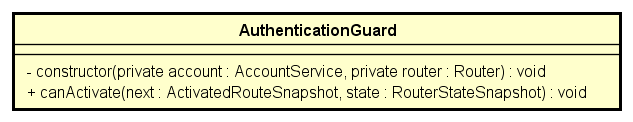
\includegraphics[scale=0.8]{res/sections/SpecificaFrontEnd/Services/Disegnetti/authenticationguard.png}
	\caption{Diagramma della classe AuthenticationGuard}
\end{figure}

\begin{itemize}
	\item \textbf{Descrizione:}\\
	Servizio che permette la verifica dell'utente durante l'autenticazione.
	
	\item \textbf{Utilizzo:}\\
	Utilizzato per verificare l'autenticazione dell'utente
	\item \textbf{Metodi:}
		\begin{itemize}
			\item \emph{-constructor( private account: AccountService, private router: Router)}\\
    		Costruttore della classe\\
    		\textbf{Parametri:}
    		\begin{itemize}
    			\item \emph{account: AccountService}\\
    			Crea un istanziazione di AccountService
    			\item \emph{router: Router}\\
    			Crea un istanziazione di Router
    		\end{itemize}
    		\item \emph{+canActivate(next: ActivatedRouteSnapshot, state: RouterStateSnapshot)}\\
    		\\
    		\textbf{Parametri:}
    		\begin{itemize}
    			\item \emph{next: ActivatedRouteSnapshot}\\
    			Un metodo dell'interfaccia
    			\item \emph{state: RouterStateSnapshot}\\
    			Un booleano dell'interfaccia
    		\end{itemize}
		\end{itemize}
\end{itemize}